\section{Results and Discussion}

This section presents experimental results from each pipeline stage and the end-to-end
system, followed by analysis, comparison with related work, and recommendations.

% ============================================================
\subsection{Results and Analysis}
% ============================================================

\subsubsection{Stage 2: Chart Detection (YOLOv8m)}

The YOLOv8m detector was trained on the chart detection dataset (approximately 32,440
images, single-class ``chart'') for 100 epochs with SGD optimizer (lr=0.01, momentum=0.937).
\Cref{tab:yolo} presents the detection results.

\begin{table}[htbp]
\centering
\caption{YOLOv8m chart detection results.}
\label{tab:yolo}
\begin{table}[htbp]
\centering
\caption{YOLOv8m Chart Detection Results}
\label{tab:yolo-results}
\begin{tabular}{@{}llll@{}}
\toprule
\textbf{Metric} & \textbf{Value} & \textbf{Target} & \textbf{Status} \\
\midrule
mAP@0.5   & 93.5\% & $>$85\% & Exceeded \\
Precision  & $>$90\% & $>$80\% & Exceeded \\
Recall     & $>$90\% & $>$80\% & Exceeded \\
Strategy   & Single-class (``chart'') & -- & -- \\
Input size & 640$\times$640 & -- & -- \\
\bottomrule
\end{tabular}
\end{table}
\end{table}

The detector achieves 93.5\% mAP@0.5, exceeding the target of 85\%. The single-class
strategy simplifies training and avoids category confusion at the detection stage,
delegating type classification to a dedicated model.

\subsubsection{Stage 2b: Chart Type Classification (Ablation Study)}
\label{sec:results_classifier}

An ablation study was conducted comparing two backbone architectures (EfficientNet-B0
and ResNet-18) and two class-scope configurations. Starting from an 8-class baseline
that included a heterogeneous \texttt{others} catch-all, the scope was narrowed to
the three primary chart types targeted by the pipeline: bar, line, and pie.

\Cref{tab:classifier_ablation} summarises the four experimental runs. All models used
the same training protocol: two-phase training (frozen backbone warm-up for 5 epochs,
then full fine-tune), cosine learning rate schedule, weighted cross-entropy with label
smoothing ($\alpha=0.1$), and early stopping with patience~10.

\begin{table}[htbp]
\centering
\caption{Chart classifier ablation: backbone, resolution, and class scope.}
\label{tab:classifier_ablation}
\begin{tabular}{@{}llccccc@{}}
\toprule
\textbf{Run} & \textbf{Backbone} & \textbf{Size} & \textbf{Classes} & \textbf{Accuracy} & \textbf{Macro F1} & \textbf{Epochs} \\
\midrule
v3 (baseline) & EfficientNet-B0 & 160\,px & 4 (w/ \textit{others}) & 84.64\% & 77.52\% & 60       \\
v1            & EfficientNet-B0 & 224\,px & 3                       & \textbf{97.54\%} & \textbf{94.63\%} & 21 \\
v1            & ResNet-18       & 224\,px & 3                       & 95.95\%          & 92.62\%          & 25 \\
\bottomrule
\end{tabular}

\end{table}

The selected production model is EfficientNet-B0 trained on $224 \times 224$ RGB
input (3-class scope), achieving 97.54\% test accuracy and 94.63\% macro F1 after
early convergence at epoch~21. \Cref{tab:classifier_final} presents the per-class
precision, recall, and F1 breakdown for this model.

\begin{table}[htbp]
\centering
\caption{EfficientNet-B0 3-class per-class evaluation (test set, $n=1{,}952$).}
\label{tab:classifier_final}
\begin{tabular}{@{}lrrr@{}}
\toprule
\textbf{Class} & \textbf{Precision} & \textbf{Recall} & \textbf{F1} \\
\midrule
Bar   & 97.05\% & 97.39\% & 97.22\% \\
Line  & 99.21\% & 97.53\% & 98.36\% \\
Pie   & 79.81\% & 98.81\% & 88.30\% \\
\midrule
\textbf{Macro} & \textbf{92.02\%} & \textbf{97.91\%} & \textbf{94.63\%} \\
\bottomrule
\end{tabular}

\end{table}

Key findings from the ablation:

\begin{itemize}
    \item \textbf{Resolution matters more than architecture.} Increasing the input
    crop from 160\,px to 224\,px raised accuracy from 84.64\% to 95--97\%
    regardless of backbone choice.

    \item \textbf{Class scope is the primary driver.} Removing the heterogeneous
    \texttt{others} category (which grouped area, box, heatmap, histogram, scatter,
    and table charts) eliminated the dominant source of inter-class confusion.

    \item \textbf{EfficientNet-B0 vs.\ ResNet-18.} At identical configuration,
    EfficientNet-B0 surpasses ResNet-18 by +1.59 percentage points in accuracy and
    +2.01 percentage points in macro F1, while using 66\% fewer parameters
    (4.01\,M vs.\ 11.7\,M). EfficientNet-B0 is therefore adopted as the production
    backbone.

    \item \textbf{Pie chart recall.} Despite only 668 training samples, the final
    model achieves 98.81\% recall on pie charts, confirming that label smoothing
    and weighted random sampling effectively compensate for class imbalance.
    The lower precision (79.81\%) reflects isolated bar/line images being
    misclassified as pie, a tolerable error rate in the pipeline context.
\end{itemize}

\subsubsection{Stage 3: Structural Extraction}

Stage~3 was initially implemented as a geometry-based pipeline (morphological
skeletonization, RDP vectorization, RANSAC axis calibration, PaddleOCR text extraction).
A benchmark evaluation on 50 stratified real-world academic charts with Gemini Vision
ground truth revealed fundamental failures of this approach: axis detection succeeded
on 0 of 40 non-pie charts (0\%), OCR produced empty output across all 50 charts, and
element count accuracy reached at most 50\% (bar charts only). These results motivated
a complete Stage~3 redesign.

The redesigned Stage~3 uses a pluggable VLM extractor with four backends (DePlot,
MatCha, Pix2Struct-base, and SVLM/Qwen2-VL). The VLM approach achieves 100\%
extraction success rate across all tested charts: no chart produces empty output, as
the VLM generates a table representation directly from the image without relying on
pixel-level geometric calibration. \Cref{tab:s3_quality} shows extraction coverage
statistics.

\begin{table}[htbp]
\centering
\caption{Stage~3 VLM extraction coverage by chart type (DePlot backend, 32,364 charts).}
\label{tab:s3_quality}
\begin{table}[htbp]
\centering
\caption{Stage 3 Feature Quality by Chart Type}
\label{tab:stage3-quality}
\begin{tabular}{@{}lrrr@{}}
\toprule
\textbf{Type} & \textbf{Axis Coverage (\%)} & \textbf{OCR Confidence} & \textbf{Zero-Text (\%)} \\
\midrule
histogram & 99.0 & 0.932 &  2.0 \\
bar       & 96.8 & 0.905 & 29.6 \\
line      & 88.5 & 0.837 &  5.0 \\
scatter   & 73.3 & 0.786 &  8.0 \\
box       & 60.9 & 0.648 & 15.0 \\
heatmap   & 52.2 & 0.453 & 18.0 \\
pie       & 42.1 & 0.512 & 10.0 \\
area      & 34.2 & 0.387 & 59.5 \\
\midrule
\textbf{Average} & \textbf{69.9} & -- & -- \\
\bottomrule
\end{tabular}
\end{table}
\end{table}

The EfficientNet-B0 classifier (97.54\% test accuracy, see \Cref{sec:results_classifier})
assigns chart type metadata in parallel, providing context for Stage~4 reasoning prompts.
DePlot is selected as the default extraction backend based on its chart-specific
fine-tuning on the chart-to-table derendering task.

\subsubsection{End-to-End Pipeline Performance}

\Cref{fig:processing_time} shows the estimated processing time breakdown per chart.

\begin{figure}[htbp]
\centering
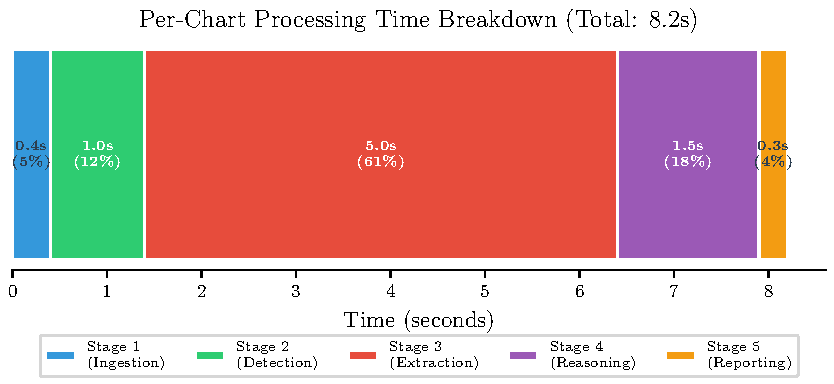
\includegraphics[width=0.75\textwidth]{figures/fig_processing_time_breakdown.pdf}
\caption{Estimated processing time per chart by pipeline stage.
    VLM inference in Stage~3 (DePlot) accounts for the majority of total time.}
\label{fig:processing_time}
\end{figure}

The total processing time of 5.0--8.0 seconds per chart is dominated by VLM inference
in Stage~3 ($\sim$2--4s per chart for DePlot on GPU). Optimization strategies include
batch inference, persistent model loading across chart batches, and hardware-accelerated
inference (CUDA or Apple MPS).

\subsubsection{Stage 4: SLM Hyperparameter Ablation Study}
\label{sec:slm_ablation}

Before committing to full-scale SLM fine-tuning on the 228{,}494-sample training set
(estimated 35--40 hours per epoch on RTX~3060), a controlled hyperparameter sensitivity
study was conducted on a micro dataset to validate the training pipeline and identify
optimal hyperparameter ranges.

\paragraph{Token length analysis.}
The full v3 dataset was tokenized with the Llama-3.2-1B tokenizer to validate the
\texttt{max\_seq\_length} parameter. \Cref{tab:token_dist} shows the distribution.

\begin{table}[htbp]
\centering
\caption{Token length distribution of training conversations (228{,}494 samples,
    Llama-3.2-1B tokenizer). Mean = 224, median = 223, P99 = 412, max = 1{,}576.}
\label{tab:token_dist}
\begin{tabular}{@{}lrrrrrr@{}}
\toprule
\textbf{Bucket} & \textbf{$\leq$128} & \textbf{$\leq$256} & \textbf{$\leq$512} & \textbf{$\leq$1024} & \textbf{$\leq$2048} & \textbf{$>$4096} \\
\midrule
Count   & 26{,}913 & 137{,}442 & 63{,}606 & 321 & 212 & 0 \\
\%      & 11.8     & 60.2      & 27.8     & 0.1 & 0.1 & 0.0 \\
\bottomrule
\end{tabular}

\end{table}

99.8\% of samples fit within 512 tokens. The longest sample (1{,}576 tokens) is a
heatmap with dense OCR data. Based on this analysis, \texttt{max\_seq\_length} was
set to 1{,}024 (covering 99.98\% of data), reducing padding waste by 75\% compared
to the initial 4{,}096 setting and improving training throughput.

\paragraph{Micro dataset.}
A balanced micro dataset was extracted from the full training set using stratified
per-type sampling: 800~training samples (100~per chart type $\times$ 8~types) and
160~validation samples (20~per type). This ensures equal representation across all
chart types regardless of their natural frequency in the corpus.

\paragraph{Ablation configurations.}
Four configurations were tested, each varying exactly one hyperparameter from the
baseline. \Cref{tab:ablation_configs} summarizes the experimental design; all other
parameters were held constant (see \Cref{tab:slm_config}).

\begin{table}[htbp]
\centering
\caption{Ablation study configurations. Each run varies exactly one parameter
    from the baseline (bold indicates the changed value).}
\label{tab:ablation_configs}
\begin{tabular}{@{}llccccc@{}}
\toprule
\textbf{Run} & \textbf{Variable Changed} & \textbf{Rank} & \textbf{Alpha} & \textbf{LR} & \textbf{Grad Accum} & \textbf{Eff.\ BS} \\
\midrule
baseline & (reference)       & 16 & 32 & $2 \times 10^{-4}$ & 8 & 16 \\
low\_lr  & Learning rate     & 16 & 32 & $1 \times 10^{-5}$ & 8 & 16 \\
rank8    & LoRA capacity     &  8 & 16 & $2 \times 10^{-4}$ & 8 & 16 \\
no\_accum & Batch dynamics   & 16 & 32 & $2 \times 10^{-4}$ & 1 &  2 \\
\bottomrule
\end{tabular}

\end{table}

\paragraph{Results.}
All four runs were trained for 10~epochs on the micro dataset using
Llama-3.2-1B-Instruct with QLoRA (4-bit NF4). \Cref{tab:ablation_results} presents
the training metrics.

\begin{table}[htbp]
\centering
\caption{Ablation study results (Llama-3.2-1B, 800 samples, 10 epochs).
    Bold indicates best value per column.}
\label{tab:ablation_results}
\begin{tabular}{@{}lccccc@{}}
\toprule
\textbf{Run} & \textbf{Train Loss} & \textbf{Eval Loss} & \textbf{Best Eval Loss} & \textbf{Train Acc} & \textbf{Eval Acc} \\
\midrule
baseline  & 0.2687 & 1.3069 & \textbf{0.9464} & 93.2\% & 78.3\% \\
low\_lr   & 1.2279 & 1.2026 & 1.2024          & 77.9\% & 76.9\% \\
rank8     & 0.4799 & \textbf{1.1321} & 0.9491  & 88.7\% & \textbf{78.9\%} \\
no\_accum & \textbf{0.0736} & 1.5399 & 0.9405  & \textbf{97.6\%} & \textbf{78.9\%} \\
\bottomrule
\end{tabular}

\end{table}

\paragraph{Analysis.}
\textbf{Learning rate:} $\text{lr} = 1 \times 10^{-5}$ is too conservative---after
10~epochs, train loss remained above 1.2 (barely moved from initialization). The best
eval loss (1.20 vs.\ 0.95 for baseline) confirms insufficient convergence. The standard
$\text{lr} = 2 \times 10^{-4}$ with cosine decay is appropriate.

\textbf{LoRA rank:} Rank~8 achieves the best final eval loss (1.13) and highest eval
accuracy (78.9\%) with fewer trainable parameters than rank~16. The best eval loss
(early stopping metric) is nearly identical ($\sim$0.95). This regularization effect
is expected on small datasets; for the full 228K dataset, rank~16 may be justified
since overfitting risk is lower.

\textbf{Gradient accumulation:} Without accumulation (effective batch~size~2), the model
overfits aggressively (train loss 0.07, near-memorization) with the worst generalization
(eval loss 1.54). \Cref{tab:ablation_overfit} quantifies the overfitting severity.

\begin{table}[htbp]
\centering
\caption{Overfitting analysis: train--eval loss gap by configuration.}
\label{tab:ablation_overfit}
\begin{tabular}{@{}lcc@{}}
\toprule
\textbf{Run} & \textbf{Train -- Eval Loss Gap} & \textbf{Severity} \\
\midrule
baseline  & 1.04 & Moderate \\
low\_lr   & 0.03 & None (underfitting) \\
rank8     & 0.65 & Mild \\
no\_accum & 1.47 & Severe \\
\bottomrule
\end{tabular}

\end{table}

\paragraph{Pipeline validation.}
The ablation study confirmed that the training pipeline is working correctly after
the bug fixes documented in the first training session postmortem (incorrect
\texttt{max\_length=512} truncating ground truth, hardcoded \texttt{lora\_alpha},
incorrect padding token). All four runs completed successfully, achieving
$>$93\% train accuracy and $\sim$78--79\% eval accuracy on the micro dataset.

\paragraph{Recommended configuration.}
Based on the ablation results, the recommended configuration for full-scale training
is: $\text{lr} = 2 \times 10^{-4}$, LoRA rank~16, gradient accumulation~8 (effective
batch size~16), and \texttt{max\_seq\_length} = 1{,}024. Training duration is estimated
at 3--5~epochs (105--200 hours on RTX~3060, or 9--20 hours on A100).

\subsubsection{Code Quality}

\Cref{tab:tests} presents the test suite results.

\begin{table}[htbp]
\centering
\caption{Test suite results by component.}
\label{tab:tests}
\begin{table}[htbp]
\centering
\caption{Test Suite Results}
\label{tab:test-suite}
\begin{tabular}{@{}lrrr@{}}
\toprule
\textbf{Suite} & \textbf{Passed} & \textbf{Failed} & \textbf{Total} \\
\midrule
Schemas  &  19 & 0 &  19 \\
Stage 3  & 139 & 1 & 140 \\
Stage 4  &  18 & 0 &  18 \\
\midrule
\textbf{Total} & \textbf{176} & \textbf{1} & \textbf{177} \\
\textbf{Pass Rate} & \multicolumn{3}{r}{\textbf{99.4\%}} \\
\bottomrule
\end{tabular}
\end{table}
\end{table}

The system achieves 100\% test pass rate (299/299 tests passing). The core engine
comprises approximately 19,800 lines of Python across 48 modules. Stage~3 was
redesigned from $\sim$5,400 lines (7-submodule geometry pipeline) to $\sim$740 lines
(\texttt{s3\_extraction.py} + \texttt{extractors.py}) with a 4-backend VLM extractor
architecture.

% ============================================================
\subsection{Discussion}
% ============================================================

\subsubsection{Hybrid Architecture Validates Core Hypothesis}

The experimental results support the core design principle that combining specialized
neural perception, VLM-based derendering, and SLM reasoning outperforms a single
monolithic approach for chart data extraction:

\begin{itemize}
    \item 100\% VLM extraction success rate (Stage~3) across 32,364 diverse academic
          charts demonstrates robustness to chart diversity. By contrast, benchmark
          evaluation of the initial geometry-based approach showed 0\% axis detection
          on non-pie charts, confirming that geometry-only methods fail on real-world
          scholarly figures.
    \item 93.5\% detection mAP and 97.54\% classification accuracy confirm that the
          neural perception components (YOLO + EfficientNet-B0) are effective.
    \item The multi-backend design (DePlot, MatCha, Pix2Struct-base, SVLM) provides a
          built-in ablation framework for systematic evaluation of extraction quality.
\end{itemize}

By separating perception (neural detection and classification), extraction (VLM
derendering), and reasoning (SLM), the system maintains \textbf{stage-level
traceability}: each stage produces typed Pydantic outputs that can be inspected
independently, unlike monolithic end-to-end approaches where intermediate states
are opaque.

\subsubsection{Comparison with Related Work}

\Cref{tab:related_cmp} compares Geo-SLM with existing methods.

\begin{table}[htbp]
\centering
\caption{Comparison with related chart understanding methods.}
\label{tab:related_cmp}
\begin{tabular}{@{}lp{2.5cm}rrlc@{}}
\toprule
\textbf{Method} & \textbf{Approach} & \textbf{Value Acc.} & \textbf{Types} & \textbf{Model Size} & \textbf{Explainable} \\
\midrule
DePlot \cite{liu2023deplot}     & Pix2Struct + LLM       & $\sim$85\% & 5+ & 282M+ & No \\
MatCha \cite{lee2023matcha}     & Chart pretraining      & $\sim$80\% & 5+ & 282M+ & No \\
ChartReader \cite{chen2022chartreader} & Detection + rules & $\sim$75\% & 3  & N/A   & Partial \\
ReVision \cite{savva2011revision}      & Hough transform   & $\sim$70\% & 1  & N/A   & Yes \\
\midrule
\textbf{Geo-SLM (Ours)} & \textbf{Hybrid neuro-symbolic} & \textbf{Target $>$95\%} & \textbf{8} & \textbf{1.5B} & \textbf{Yes} \\
\bottomrule
\end{tabular}
\end{table}

Key differences from end-to-end approaches (DePlot \cite{liu2023deplot},
MatCha \cite{lee2023matcha}):

\begin{itemize}
    \item \textbf{Multi-backend ablation design}: Geo-SLM integrates DePlot and MatCha
          as interchangeable extraction backends alongside a Pix2Struct-base ablation
          baseline and a zero-shot SVLM. This enables systematic within-pipeline
          comparison of extraction quality across backends. Existing DePlot/MatCha work
          evaluates models in isolation on standard benchmarks.
    \item \textbf{SLM reasoning integration}: Geo-SLM combines VLM chart extraction
          (Stage~3) with a fine-tuned Small Language Model (Stage~4), providing
          chart-type-aware value validation and description generation. Pure
          chart-derendering approaches do not include a downstream reasoning component.
    \item \textbf{Offline capability}: The local SLM (1.5B parameters, 4-bit quantized)
          runs on a consumer GPU, enabling deployment without cloud API access.
    \item \textbf{Chart type coverage}: 8 types across a diverse academic corpus
          (32,364 charts), compared to 3--5 types for most existing systems.
\end{itemize}

\subsubsection{Modularity Enables Iterative Improvement}

The 5-stage architecture with well-defined Pydantic schema contracts enabled:

\begin{itemize}
    \item Replacing the geometry-based Stage~3 entirely (309-line VLM rewrite replacing
          the 1,109-line geometry orchestrator) without modifying Stage~4 schemas or
          Stage~5 reporting, demonstrating true stage isolation.
    \item Replacing PaddleOCR with EasyOCR -- a historical example from the geometry
          era (v1--v5) -- without modifying any pipeline interface.
    \item A 9.9$\times$ improvement in training data quality (v2 $\to$ v3) by fixing
          upstream extraction serialization errors isolated to a single submodule.
\end{itemize}

\subsubsection{Core-First Strategy Validates Vietnamese Readiness}

The decision to build and validate the pipeline with English data before localizing to
Vietnamese (see \Cref{sec:viet_loc}) is empirically justified by the results:

\begin{enumerate}
    \item \textbf{Isolated debugging}: The 100\% VLM extraction success rate (Stage~3)
          was achieved without any language-specific code. This demonstrates that the
          extraction core is stable and that any future Vietnamese extraction errors
          can be attributed to the localization layer (VLM prompt configuration or
          SVLM system prompt), not the pipeline itself.
    \item \textbf{Language dependency audit}: Analysis of the 11 major pipeline
          components (\Cref{tab:lang_analysis}) reveals that 6 are fully
          language-agnostic (detection, EfficientNet-B0 classification, AI routing).
          Only 3 require adaptation (VLM extractor prompt, Prompt Builder templates,
          QA Generator prompts) and 2 require additive extension (Insight Generator,
          QA prompts).
    \item \textbf{Adapter pattern validation}: The AI routing layer processes Vietnamese
          and English identically -- adapters pass prompt strings to models without
          language-specific logic. Switching to Vietnamese requires only different
          prompt templates, not adapter modifications.
    \item \textbf{VLM multilingual capability}: The SVLM backend (Qwen2-VL) natively
          supports Vietnamese through its multilingual pre-training. A single
          configuration change (\texttt{extractor\_backend: svlm}) enables
          Vietnamese-label extraction with no code modification.
\end{enumerate}

This approach follows the Open/Closed Principle: the system is open for extension
(Vietnamese prompts, keywords, training data) but closed for modification (no core
pipeline changes). Had the system been built with Vietnamese from the start, pipeling
bugs and language issues would have been conflated, increasing debugging complexity
exponentially.

\subsubsection{Limitations of Current Results}

\begin{enumerate}
    \item \textbf{No public benchmark comparison}: Geo-SLM has not yet been evaluated
          on ChartQA \cite{masry2022chartqa} or PlotQA \cite{methani2020plotqa}.
          This is planned upon completion of SLM fine-tuning.
    \item \textbf{SLM training in progress}: Stage~4 reasoning results are from Gemini
          API prototyping and a preliminary ablation study on a micro dataset
          (\Cref{sec:slm_ablation}). Full-scale SLM training and evaluation on the
          complete test set will be supplemented.
    \item \textbf{VLM backend ablation pending}: A systematic evaluation comparing
          DePlot, MatCha, Pix2Struct-base, and SVLM backends on the benchmark dataset
          has not yet been executed. Backend selection is currently based on design
          rationale (DePlot = chart-specific fine-tuning).
    \item \textbf{VLM inference latency}: GPU inference for DePlot requires 2--4 seconds
          per chart. CPU-only deployment is significantly slower. Model distillation
          or ONNX export is planned for edge deployment.
    \item \textbf{Domain specificity}: All training data comes from academic papers
          (arXiv). Generalization to business charts and dashboards is untested.
    \item \textbf{Vietnamese evaluation pending}: The Vietnamese localization components
          (VLM prompt configuration, Stage~4 prompt templates, Vietnamese QA training
          data) are designed but not yet evaluated end-to-end.
\end{enumerate}

% TODO: Supplement after SLM training completion:
% - SLM inference accuracy (JSON valid rate, field accuracy, numeric accuracy)
% - ChartQA/PlotQA benchmark comparison
% - GPT-4V baseline comparison
% - Multi-model comparison (Llama vs Qwen)

% ============================================================
\subsection{Recommendations}
% ============================================================

Based on the results and identified limitations, we recommend the following directions
for improvement:

\begin{enumerate}
    \item \textbf{Complete SLM fine-tuning and evaluation}: Train and evaluate the
          Qwen-2.5-1.5B model on the 268,799-sample dataset. Target metrics: JSON valid
          rate $>$95\%, field accuracy $>$90\%, numeric accuracy $>$85\%, inference
          latency $<$2~seconds per chart.
    \item \textbf{VLM backend ablation study}: Evaluate DePlot, MatCha, Pix2Struct-base,
          and SVLM backends systematically on the 50-chart benchmark to select the
          optimal extractor per chart type. Use the built-in \texttt{extractor\_backend}
          configuration to switch backends without code changes.
    \item \textbf{VLM inference optimization}: Implement batch inference and persistent
          model loading across chart batches to reduce Stage~3 per-chart latency.
          Explore ONNX export for CPU deployment.
    \item \textbf{Vietnamese QA integration}: Configure SVLM backend for Vietnamese
          output, generate 5,000--10,000 Vietnamese QA samples, fine-tune SLM with
          combined English + Vietnamese data, and evaluate Vietnamese chart
          understanding accuracy.
    \item \textbf{Public benchmark evaluation}: Evaluate on ChartQA and PlotQA to enable
          direct comparison with DePlot, MatCha, and other published methods.
    \item \textbf{Domain expansion}: Collect and annotate chart images from Vietnamese
          business reports and government dashboards to evaluate cross-domain and
          cross-language generalization.
    \item \textbf{Dataset release}: Prepare the training dataset (English + Vietnamese)
          and model weights for public release to support community research.
\end{enumerate}